\documentclass[conference]{IEEEtran}
% Build: pdflatex main && bibtex main && pdflatex main && pdflatex main
% All numbers in \res... macros, the tables and the abstract are generated by
% `make report` into paper/generated/ from results/*.json.
\usepackage[T1]{fontenc}
\usepackage{amsmath,amssymb}
\usepackage{graphicx}
\usepackage{booktabs}
\usepackage{adjustbox}
\usepackage{url}
\usepackage{xcolor}
\usepackage{cite}
\graphicspath{{../figures/}}
% several floats per page, so tables sit next to their text instead of trailing the paper
\setcounter{topnumber}{3}
\setcounter{bottomnumber}{2}
\setcounter{totalnumber}{5}
\setcounter{dbltopnumber}{3}
\renewcommand{\topfraction}{0.9}
\renewcommand{\bottomfraction}{0.6}
\renewcommand{\textfraction}{0.08}
\renewcommand{\floatpagefraction}{0.75}
\renewcommand{\dbltopfraction}{0.9}
\renewcommand{\dblfloatpagefraction}{0.75}
% generated by rotorfault.experiments.report -- do not edit
\newcommand{\resEOnePassiveMaxdevFiveZeroCm}{28}
\newcommand{\resEOneEstMaxdevFiveZeroCm}{4.3}
\newcommand{\resEOneOracleMaxdevFiveZeroCm}{4.3}
\newcommand{\resEOnePassiveLostSevenZero}{3}
\newcommand{\resEOnePassiveLostNineZero}{8}
\newcommand{\resEOneN}{8}
\newcommand{\resEOneEstLostAny}{0}
\newcommand{\resEOneEstTotal}{80}
\newcommand{\resEOneEstMaxdevNineZeroCm}{27}
\newcommand{\resETwoNFault}{200}
\newcommand{\resETwoDetected}{200}
\newcommand{\resETwoIsolationPct}{100}
\newcommand{\resETwoDelayMedianMs}{30}
\newcommand{\resETwoDelayPNineFiveMs}{58}
\newcommand{\resETwoDelayLowBinMedianMs}{51}
\newcommand{\resETwoDelayHighBinMedianMs}{24}
\newcommand{\resETwoLoeAbsErrMedianPts}{1.5}
\newcommand{\resETwoLoeAbsErrPNineFivePts}{4.8}
\newcommand{\resETwoFalseAlarms}{0}
\newcommand{\resETwoFreeMinutes}{32}
\newcommand{\resETwoNFree}{100}
\newcommand{\resETwoNoiseMaxScale}{8}
\newcommand{\resETwoNoiseMaxDeg}{14}
\newcommand{\resETwoNoiseMaxDelayMs}{25}
\newcommand{\resETwoNoiseMaxIsolationPct}{100}
\newcommand{\resETwoNoiseMaxDetected}{40}
\newcommand{\resETwoNoiseMaxN}{40}
\newcommand{\resETwoNoiseMaxFa}{0}
\newcommand{\resEThreeRmseBeforeCm}{3.5}
\newcommand{\resEThreePassiveTransientCm}{18}
\newcommand{\resEThreeEstTransientCm}{3.5}
\newcommand{\resEThreePassiveMaxdevCm}{25}
\newcommand{\resEThreeEstMaxdevCm}{6.8}
\newcommand{\resEFourN}{32}
\newcommand{\resEFourPassiveLost}{32}
\newcommand{\resEFourPassiveTtlS}{0.3}
\newcommand{\resEFourEstLost}{0}
\newcommand{\resEFourOracleLost}{0}
\newcommand{\resEFourEstMaxdevCm}{38}
\newcommand{\resEFourOracleMaxdevCm}{22}
\newcommand{\resEFourEstSettledCm}{7.6}
\newcommand{\resEFourEstSpin}{23}
\newcommand{\resEFourEstSwitchMs}{62}
\newcommand{\resEFourEstTiltDeg}{42}
\newcommand{\resEFiveN}{24}
\newcommand{\resEFiveEstLost}{0}
\newcommand{\resEFivePassiveLost}{24}
\newcommand{\resEFiveEstMaxdevCm}{39}
\newcommand{\resEFiveEstSettledCm}{18}
\newcommand{\resESevenNoBaselineFaRuns}{1}
\newcommand{\resESevenNoBaselineFaPre}{1}
\newcommand{\resESevenNoBaselineDelayMs}{28}
\newcommand{\resESevenNoBaselineIsolationPct}{100}
\newcommand{\resESevenNoAdaptiveFaRuns}{0}
\newcommand{\resESevenNoAdaptiveFaPre}{0}
\newcommand{\resESevenNoAdaptiveDelayMs}{25}
\newcommand{\resESevenNoAdaptiveIsolationPct}{100}
\newcommand{\resESevenSingleCusumFaRuns}{0}
\newcommand{\resESevenSingleCusumFaPre}{0}
\newcommand{\resESevenSingleCusumDelayMs}{61}
\newcommand{\resESevenSingleCusumIsolationPct}{100}
\newcommand{\resESevenNFree}{30}
\newcommand{\resESevenNFault}{60}
\newcommand{\resSitlNTotal}{110}
\newcommand{\resSitlNCal}{24}
\newcommand{\resSitlNFree}{24}
\newcommand{\resSitlFreeMin}{22}
\newcommand{\resSitlFa}{0}
\newcommand{\resSitlFaNoad}{0}
\newcommand{\resSitlPartN}{40}
\newcommand{\resSitlPartDet}{40}
\newcommand{\resSitlPartIso}{40}
\newcommand{\resSitlPartLoeLo}{19}
\newcommand{\resSitlPartLoeHi}{48}
\newcommand{\resSitlPartDelayMed}{120}
\newcommand{\resSitlPartDelayPNineFive}{128}
\newcommand{\resSitlPartLoeErr}{0.5}
\newcommand{\resSitlPartLoeErrPNineFive}{3.9}
\newcommand{\resSitlPartDelayNoad}{40}
\newcommand{\resSitlPartIsoNoad}{38}
\newcommand{\resSitlPartPxFour}{0}
\newcommand{\resSitlPartHeld}{21}
\newcommand{\resSitlPartDescended}{18}
\newcommand{\resSitlPartFlipped}{1}
\newcommand{\resSitlPartHeldLow}{15}
\newcommand{\resSitlPartNLow}{16}
\newcommand{\resSitlPartHeldHigh}{6}
\newcommand{\resSitlPartNHigh}{24}
\newcommand{\resSitlBinEdge}{35}
\newcommand{\resSitlCompN}{16}
\newcommand{\resSitlCompDet}{16}
\newcommand{\resSitlCompIso}{16}
\newcommand{\resSitlCompDelayMed}{132}
\newcommand{\resSitlCompDelayPNineFive}{141}
\newcommand{\resSitlCompDelayNoad}{20}
\newcommand{\resSitlCompIsoNoad}{14}
\newcommand{\resSitlCompPxFour}{16}
\newcommand{\resSitlCompPxFourMs}{664}
\newcommand{\resSitlCompFlipMs}{486}
\newcommand{\resSitlCompFlipped}{16}
\newcommand{\resSitlCompBefore}{16}
\newcommand{\resSitlCompPxFourAfter}{16}
\newcommand{\resSitlDelayMs}{4}
\newcommand{\resSitlPxoffN}{4}
\newcommand{\resSitlPxoffFlipped}{4}
\newcommand{\resSitlPxoffPxFourMs}{660}
\newcommand{\resSitlPxdefN}{2}
\newcommand{\resSitlPxdefEffective}{0}


\begin{document}

\title{Detect, Isolate, Recover: Rotor-Fault Tolerance\\for a 5-inch Quadrotor (Simulation Study)}
\author{\IEEEauthorblockN{Rami Kronbi}
\IEEEauthorblockA{Independent researcher\\Code and data: \texttt{rotor-fault-recovery} (MIT license)}}
\maketitle

\begin{abstract}
We study rotor-fault tolerance for a simulated 5-inch FPV-class quadrotor (0.64 kg, thrust-to-weight 3.6) with sensor noise, a 10 ms motion-capture latency, parameter uncertainty and light turbulence. An online estimator of the four rotor effectiveness factors (filtered rigid-body regression, Kalman filter) feeds a bank of CUSUM tests for detection and isolation; a supervisor then either re-allocates thrust with the estimated effectiveness (partial loss) or, when a rotor can no longer carry its share of the weight, switches to a yaw-relaxed controller in the spirit of Mueller and D'Andrea (2014) that spins the vehicle about a tilted primary axis (gain-scheduled LQR on the reduced attitude). In 200 Monte-Carlo runs with 20-90 \% loss of effectiveness, all faults were detected (median delay 30 ms, 95th percentile 58 ms) and all were isolated to the correct rotor, with a median magnitude error of 1.5 percentage points; no false alarm occurred in 32 min of fault-free flight. With a 50 \% loss in hover the median peak deviation drops from 28 cm (passive) to 4.3 cm. After a complete rotor loss in hover the passive controller lost the vehicle in 32/32 runs (median 0.30 s), while the proposed pipeline recovered 32/32 with a median peak deviation of 38 cm and a spin of 23 rad/s; it also recovered 24/24 complete losses during a 3.3 m/s figure-eight. These are simulation results with assumed, not identified, parameters; in the robustness sweeps complete-loss recovery started to fail at an actuator delay of 24 ms (2 ms assumed), a motor time constant of 80 ms (25 ms assumed) and 3x the default turbulence. In 110 PX4 software-in-the-loop flights of a Gazebo x500, replayed offline with parameters read from the simulator's model files, the same diagnoser detected and isolated all 40 injected partial losses (19-48 \%, median delay 120 ms) and all 16 complete losses (median 132 ms), with no false alarm in 22 min of fault-free flight; PX4's own failure detector flagged none of the partial losses and the complete losses only after 664 ms, once the vehicle had flipped.

\end{abstract}

\section{Introduction}
A quadrotor has as many actuators as controlled degrees of freedom, so a damaged
propeller, a prop strike or a failed motor channel cannot be compensated by redundancy.
Small FPV-class vehicles meet such faults routinely, and their flight software usually
treats them only as a reason to disarm. Fault-tolerant control (FTC) of multirotors is a
mature topic: Zhang and Jiang~\cite{zhang2008bibliographical} review reconfigurable FTC in
general, model-based actuator fault diagnosis and accommodation for quadrotors was shown by
Avram et al.~\cite{avram2017quadrotor}, and the complete loss of a rotor has been handled by
giving up yaw: Mueller and D'Andrea derived ``relaxed hover'' solutions in which the vehicle
spins about a body-fixed primary axis and controlled the reduced attitude with
LQR~\cite{mueller2014stability,mueller2016relaxed}, Lanzon et al.\ designed a controller for
the same situation~\cite{lanzon2014flight}, and Sun et al.\ used incremental nonlinear dynamic
inversion (INDI)~\cite{smeur2016adaptive} to fly a quadrotor with two opposing rotors lost at
high speed~\cite{sun2021incremental}.

This report puts the pieces together for one specific vehicle class, a 5-inch FPV quadrotor
with a thrust-to-weight ratio of 3.6, and asks three questions: how fast and how reliably can a
loss of effectiveness (LOE) be detected, isolated and quantified without RPM telemetry; how
much does acting on that estimate help compared with a passive controller and with an oracle;
and where does yaw-relaxed recovery from a complete loss break. The contribution is not a new
control law. It is an end-to-end, reproducible pipeline evaluated under sensor noise,
motion-capture latency, parameter spread and turbulence, with its failure limits reported.

\section{Model}
\textbf{Vehicle.} Position $p$ and velocity $v$ in a z-up world frame, unit quaternion attitude
$q$ (rotation $R$), body rate $\omega$ and rotor speeds $\Omega_i$:
\begin{align}
m\dot v &= -mg e_3 + R\,T e_3 - R D R^\top v - c\|v\|v + F_d,\\
J\dot\omega &= \tau(f,\dot\Omega) - \omega\times(J\omega + h_r) - K_\omega\omega + \tau_d,\\
\dot\Omega_i &= (\Omega_{\mathrm{cmd},i}-\Omega_i)/\tau_m,\quad f_i = \eta_i k_f \Omega_i^2,
\end{align}
with rotor angular momentum $h_r$, yaw reaction torque $\kappa f_i$ per rotor plus the reaction
of accelerating rotors, and turbulence $F_d,\tau_d$ (independent Ornstein--Uhlenbeck processes,
0.15\,N and $4\times10^{-3}$\,N\,m, 0.3\,s correlation). $\eta_i\in[0,1]$ is the effectiveness of
rotor $i$; a fault is a step in one $\eta_i$. Mass (0.638\,kg) and inertia
($\mathrm{diag}(1.36,2.12,3.13)\times10^{-3}$\,kg\,m$^2$) come from a lumped mass budget; arm length
0.11\,m, 5.6\,N maximum rotor thrust, $\kappa=0.015$\,m, $\tau_m=25$\,ms, rotational damping
$(2.5,2.5,2.0)\times10^{-3}$\,N\,m\,s. The true vehicle of each run is drawn around these values
(mass $\pm3\%$, inertia $\pm5\%$, $k_f$ $\pm3\%$ per rotor, $\tau_m$ $\pm10\%$, damping $\pm20\%$); the
flight software always uses the nominal model. Integration is RK4 at 1\,kHz; estimation, FDI
and control run at 500\,Hz with 2\,ms actuator transport delay.

\textbf{Sensors.} Gyro with 0.03\,rad/s white noise per sample, random-walk bias and
$\pm2000^\circ$/s range; accelerometer with 0.2\,m/s$^2$ noise and bias; motion capture at
100\,Hz with 1\,mm / 0.3$^\circ$ noise and 10\,ms latency. A complementary attitude filter and a
position/velocity Kalman filter fuse them, using time-stamped history for the delayed
motion-capture samples. Controllers and the diagnoser never see the true state.

\section{Nominal control and allocation}
The nominal controller is the geometric tracking controller on SE(3) of Lee et
al.~\cite{lee2010geometric} (z-up form), with integral action on position and attitude, tilt
limits and drag feed-forward; its SO(3) attitude error has no singularities and behaves well
for the large errors that follow a fault. Allocation solves $[T,\tau]^\top = B\,\mathrm{diag}(\eta)
f$ under $f_{\min}\le f\le f_{\max}$ in closed form with priorities: the roll/pitch torque is kept
(scaled only if infeasible), the collective is shifted by the smallest feasible amount, and the
yaw torque is scaled last.

\section{Fault detection, isolation and estimation}
\textbf{Regression.} The rotational dynamics and the body-z force balance are linear in $\eta$:
\begin{equation}
\begin{aligned}
y &\triangleq \begin{bmatrix} m a_z + D_z v_z + c\|v\|v_z\\ J\dot\omega + \omega\times(J\omega+h_r)
+K_\omega\omega - \tau_{\dot\Omega}\end{bmatrix}\\
&= B\,\mathrm{diag}(\hat f)\,\eta \triangleq \Phi\eta,
\end{aligned}
\end{equation}
where $\hat f$ are thrusts predicted from the commands through the nominal motor model and the
known delay. $\dot\omega$ comes from a 15\,Hz second-order state-variable filter of the gyro, and
every other signal of the regression passes through the same filter.

\textbf{Estimation.} A Kalman filter with a random-walk model on $\eta$ (equivalently RLS with
forgetting) tracks $\hat\eta$, projected onto $[0,1.1]$; rotors commanded near idle are frozen.
Static mismatch (3\,\% $k_f$ spread, mass error) is indistinguishable from a small LOE, so the
estimate is averaged over the initial 2.5\,s hover into a healthy baseline $\eta_{\mathrm{ref}}$.

\textbf{Detection and isolation.} Each residual row is normalised by
$\sigma_k=\sqrt{\sigma_0^2+u_k^2}$, a calibrated floor plus the residual that the assumed inertia
(5\,\%) and motor-lag (10\,\%) uncertainty can produce at that instant. A loss $\delta$ on rotor
$j$ shifts $r=(y-\Phi\eta_{\mathrm{ref}})/\sigma$ by $\delta d_j$ with the known signature
$d_j=-\Phi_{:,j}\eta_{\mathrm{ref},j}/\sigma$. With $t_j=d_j^\top r/\|d_j\|$, a bank of one-sided
CUSUM tests~\cite{page1954continuous,basseville1993detection}
\begin{equation}
g_{kj}\leftarrow\max\!\big(0,\;g_{kj}+\mu_{kj}(t_j-\mu_{kj}/2)\big),\quad \mu_{kj}=\delta_k\|d_j\|,
\end{equation}
for $\delta_k\in\{0.15,0.3,0.6\}$ approximates the GLR test for an unknown fault size
(cf.\ Lorden~\cite{lorden1971procedures}); an alarm is raised when any $g_{kj}>h_k$ and rotor
$\arg\max_j g_{kj}$ of the firing test is isolated. Because the residual is coloured and the model
inexact, $\sigma_0$ and $h_k$ are calibrated on 60 fault-free flights with seeds disjoint from all
evaluation runs: $h_k$ is twice the largest statistic observed, floored at the evidence a
design-size fault accumulates in 20\,ms. The aggressive waypoint manoeuvre is excluded from
calibration.

\section{Fault-tolerant control}
\textbf{Partial loss.} After an alarm, allocation uses $B\,\mathrm{diag}(\hat\eta)$.

\textbf{Complete loss.} If $\hat\eta_j<0.35$ for 30\,ms (below $\approx0.29$ the rotor cannot carry
a quarter of the weight), rotor $j$ is idled and a yaw-relaxed controller in the spirit
of~\cite{mueller2014stability,mueller2016relaxed} takes over. The relaxed-hover equilibrium is
computed numerically: three thrusts and a constant body rate $\bar\omega=\bar r\,\bar n/\bar n_z$
along a body-fixed axis $\bar n$ such that all torques balance (including rotor gyroscopics and
damping) and $f_T\bar n_z=mg$. The solutions form a two-parameter family; I fix the tilt of
$\bar n$ from body $z$ at $15^\circ$ and choose its azimuth to minimise the spin
(Fig.~\ref{fig:family}), giving 24\,rad/s, 69\,\% of the gyro range. The reduced dynamics -- $p$,
$q$, the two components of the axis error in the plane orthogonal to $\bar n$ (with
$\dot n=-\omega\times n$ for the desired axis expressed in the body frame) and three motor
states -- are linearised numerically about quasi-equilibria with the yaw rate frozen at 14
values between 0 and $1.3\bar r$; a discrete LQR is computed at each point and scheduled on the
measured yaw rate, as is the gyroscopic torque feed-forward. An outer position loop commands
the direction of $\bar n$ and $f_T=m\|a_{\mathrm{cmd}}\|/\bar n_z$.

\textbf{Baselines.} \emph{Passive}: nominal controller, faults ignored. \emph{Oracle}: the true
$\eta$ and onset are given to the supervisor. \emph{Estimated}: the proposed pipeline. For a given
seed, all three see the same vehicle, noise and turbulence.

\begin{figure}[t]
\centering
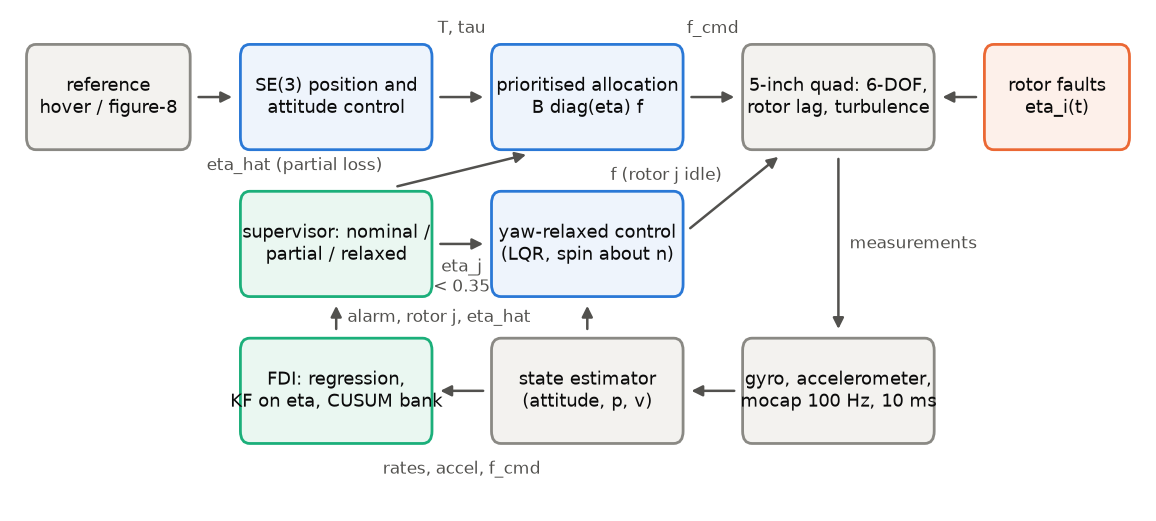
\includegraphics[width=\columnwidth]{fig_architecture.png}
\caption{Pipeline. The supervisor switches between nominal, partial-loss (re-allocation with
$\hat\eta$) and yaw-relaxed control.}
\label{fig:arch}
\end{figure}

\section{Experiments}
E1: hover, step LOE 0--90\,\% on rotor 1 at $t=2$\,s, 8 seeds per point. E2: 200 faulty runs
(random rotor, LOE $\sim\mathcal U[0.2,0.9]$, onset $\sim\mathcal U[2,5]$\,s, hover or a figure-eight
at up to 3.3\,m/s) and 100 fault-free runs of 12\,s (hover, figure-eight, aggressive waypoint
steps), plus a gyro-noise sweep (0.5--8$\times$, re-calibrated per level). E3: figure-eight with
50\,\% LOE at $t=10$\,s. E4/E5: complete loss of each rotor in hover / on the figure-eight. E6:
robustness of E4 to the true actuator delay, motor time constant, damping, inertia and
turbulence. E7: FDI ablation. A run is \emph{lost} on ground contact, tilt $>90^\circ$ or position
error $>3$\,m.

\section{Results}
\textbf{Partial loss (E1, E3).} With 50\,\% LOE in hover the median peak deviation drops from
\resEOnePassiveMaxdevFiveZeroCm\,cm (passive) to \resEOneEstMaxdevFiveZeroCm\,cm, which is the
turbulence floor (Fig.~\ref{fig:e1}, Table~\ref{tab:e1}). The passive controller recovers partial
losses eventually through its integrators but loses \resEOnePassiveLostSevenZero/\resEOneN{} runs at
70\,\% and \resEOnePassiveLostNineZero/\resEOneN{} at 90\,\%; the active pipelines lose none. Two
unexpected results: at 80\,\% the passive vehicle survives in an uncontrolled but stable yaw spin,
and at 70--80\,\% the estimated pipeline beats the oracle because the oracle idles the weakened
rotor immediately. On the figure-eight (Table~\ref{tab:e3}) the median peak deviation after a
50\,\% loss is \resEThreePassiveMaxdevCm\,cm passive and \resEThreeEstMaxdevCm\,cm estimated.

\begin{table*}[t]
\centering
\caption{E1: hover with a step loss of effectiveness on rotor 1. Hover, fault at t = 2 s. Each cell: median max deviation / median settled error (cm) over non-lost runs, (lost/total).}
\label{tab:e1}
\footnotesize
\setlength{\tabcolsep}{3pt}
\begin{adjustbox}{max width=\linewidth}
\begin{tabular}{lccc}
\toprule
LOE rotor 1 & Passive & Oracle & Estimated (proposed) \\
\midrule
20 \% & 7.6 / 2.7 (0/8) & 4.3 / 2.5 (0/8) & 4.3 / 2.2 (0/8) \\
40 \% & 18.1 / 3.3 (0/8) & 4.3 / 2.5 (0/8) & 4.3 / 2.2 (0/8) \\
60 \% & 46.1 / 5.5 (0/8) & 4.3 / 2.5 (0/8) & 4.4 / 2.2 (0/8) \\
70 \% & 73.5 / 16.1 (3/8) & 19.5 / 5.6 (0/8) & 12.9 / 5.5 (0/8) \\
80 \% & 97.7 / 31.0 (0/8) & 19.8 / 5.7 (0/8) & 18.7 / 5.5 (0/8) \\
90 \% & -- / -- (8/8) & 20.1 / 5.8 (0/8) & 27.2 / 6.2 (0/8) \\
\bottomrule
\end{tabular}
\end{adjustbox}
\end{table*}

\begin{table}[t]
\centering
\caption{E3: figure-eight tracking with a 50 \% loss. Figure-eight (peak 3.3 m/s), 50 \% LOE on rotor 1 at t = 10 s; medians over 10 seeds, cm.}
\label{tab:e3}
\footnotesize
\setlength{\tabcolsep}{3pt}
\begin{adjustbox}{max width=\linewidth}
\begin{tabular}{lccccc}
\toprule
Baseline & RMSE before & RMSE 0-3 s after & RMSE 3-10 s after & max dev. & lost \\
\midrule
Passive & 3.5 & 17.6 & 8.5 & 24.7 & 0/10 \\
Oracle & 3.5 & 3.7 & 4.0 & 7.0 & 0/10 \\
Estimated (proposed) & 3.5 & 3.5 & 3.9 & 6.8 & 0/10 \\
\bottomrule
\end{tabular}
\end{adjustbox}
\end{table}


\begin{figure}[t]
\centering
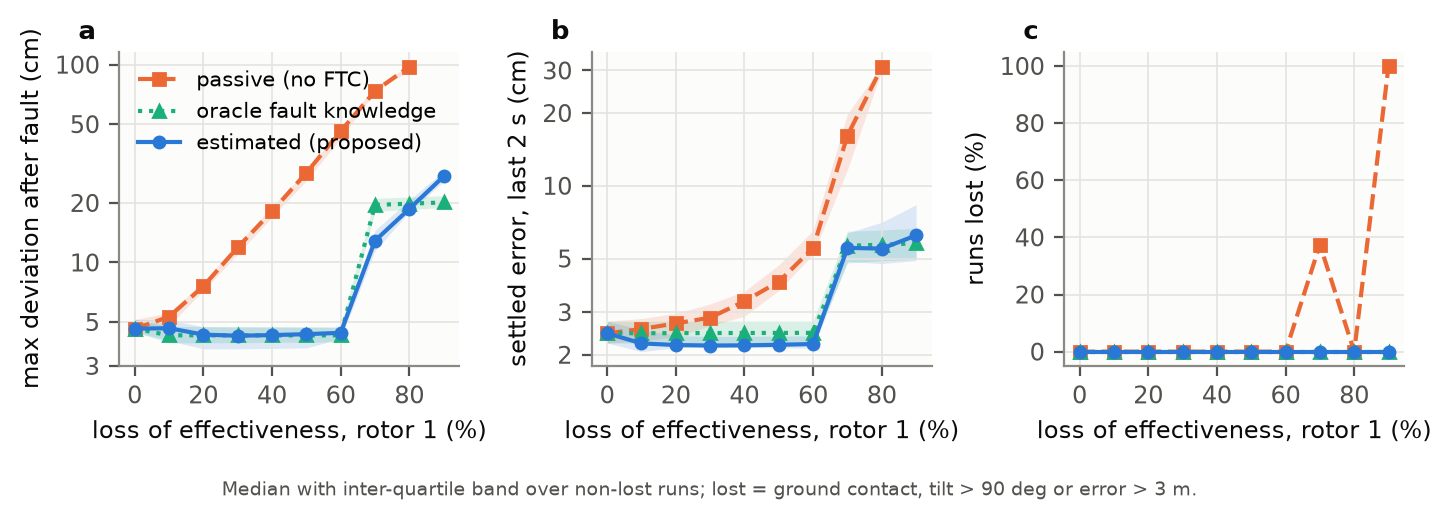
\includegraphics[width=\columnwidth]{fig_e1_hover_loe.png}
\caption{E1: peak deviation, settled error and loss rate versus LOE magnitude (median and IQR,
8 seeds).}
\label{fig:e1}
\end{figure}

\textbf{Diagnosis (E2, E7).} All \resETwoNFault{} faults were detected
(median delay \resETwoDelayMedianMs\,ms, 95th percentile \resETwoDelayPNineFiveMs\,ms; about
\resETwoDelayLowBinMedianMs\,ms for 20--35\,\% and \resETwoDelayHighBinMedianMs\,ms for 80--90\,\%),
\resETwoIsolationPct\,\% were isolated correctly and the median magnitude error was
\resETwoLoeAbsErrMedianPts{} percentage points (Fig.~\ref{fig:e2}, Table~\ref{tab:e2});
\resETwoFalseAlarms{} false alarms occurred in \resETwoFreeMinutes\,min of fault-free flight,
including aggressive waypoint steps that were not used for calibration. Up to 8$\times$ gyro noise
(14$^\circ$/s per sample), detection and isolation are essentially unchanged, with re-calibrated
thresholds and also with the 1$\times$ thresholds (Table~\ref{tab:e2noise}): in this model
turbulence and mismatch, not white gyro noise, set the residual floor. The ablation
(Table~\ref{tab:e7}) shows that without the healthy baseline static mismatch causes false alarms
(\resESevenNoBaselineFaRuns/\resESevenNFree{} fault-free runs and \resESevenNoBaselineFaPre{} faulty
run before its onset), and that a single CUSUM designed for 15\,\% roughly doubles the median delay
(\resESevenSingleCusumDelayMs{} vs.\ \resETwoDelayMedianMs\,ms). The adaptive residual scale made
no measurable difference in these tests (no false alarms without it, \resESevenNoAdaptiveDelayMs\,ms
median delay), so no benefit is claimed for it.

\begin{table}[t]
\centering
\caption{E2: fault detection and isolation Monte Carlo. 200 faulty runs (hover and figure-eight). False alarms: 0 in 32 min of fault-free flight (100 fault-free runs incl. unseen aggressive steps, plus pre-onset time of the faulty runs).}
\label{tab:e2}
\footnotesize
\setlength{\tabcolsep}{3pt}
\begin{adjustbox}{max width=\linewidth}
\begin{tabular}{lcccc}
\toprule
LOE & detected & delay ms: median (p95) & isolation & abs. LOE error, pts: median (p95) \\
\midrule
20-35 \% & 33/33 & 51 (80) & 100.0 \% & 1.7 (4.6) \\
35-50 \% & 44/44 & 37 (43) & 100.0 \% & 1.0 (4.4) \\
50-65 \% & 44/44 & 30 (35) & 100.0 \% & 1.1 (2.7) \\
65-80 \% & 46/46 & 27 (32) & 100.0 \% & 1.3 (3.7) \\
80-90 \% & 33/33 & 24 (27) & 100.0 \% & 3.8 (5.4) \\
all 20-90 \% & 200/200 & 30 (58) & 100.0 \% & 1.5 (4.8) \\
\bottomrule
\end{tabular}
\end{adjustbox}
\end{table}

\begin{table*}[t]
\centering
\caption{E2: sensitivity to gyro noise. 1x = main experiment (200 + 100 runs); other levels 40 faulty + 20 fault-free runs with residual floor and thresholds re-calibrated for that level; the second false-alarm column re-flies the 20 fault-free runs with the thresholds calibrated at 1x.}
\label{tab:e2noise}
\footnotesize
\setlength{\tabcolsep}{3pt}
\begin{adjustbox}{max width=\linewidth}
\begin{tabular}{lccccccc}
\toprule
gyro noise (deg/s) & detected & delay ms: median (p95) & isolation & abs. LOE error, pts & false alarms & false alarms, 1x thresholds & lost \\
\midrule
0.5x (0.9) & 40/40 & 18 (30) & 100.0 \% & 1.1 & 0 & 0/20 runs & 0 \\
1x (1.7) & 200/200 & 30 (58) & 100.0 \% & 1.5 & 0 & -- & 0 \\
2x (3.4) & 40/40 & 26 (34) & 100.0 \% & 1.3 & 0 & 0/20 runs & 0 \\
4x (6.9) & 40/40 & 29 (53) & 100.0 \% & 1.7 & 0 & 0/20 runs & 0 \\
8x (13.8) & 40/40 & 25 (48) & 100.0 \% & 2.0 & 0 & 0/20 runs & 0 \\
\bottomrule
\end{tabular}
\end{adjustbox}
\end{table*}

\begin{table*}[t]
\centering
\caption{E7: FDI ablation. 60 faulty + 30 fault-free runs per variant (same seeds), each variant calibrated with the same procedure; detected counts alarms after onset.}
\label{tab:e7}
\footnotesize
\setlength{\tabcolsep}{3pt}
\begin{adjustbox}{max width=\linewidth}
\begin{tabular}{lcccccc}
\toprule
FDI variant & detected & delay ms: median (p95) & isolation & |LOE err| pts & false-alarm runs (+ before onset) & lost \\
\midrule
proposed (all elements) & 60/60 & 30 (64) & 100.0 \% & 1.6 & 0/30 (+0) & 0 \\
no healthy baseline & 59/60 & 28 (63) & 100.0 \% & 1.8 & 1/30 (+1) & 0 \\
no adaptive residual scale & 60/60 & 25 (56) & 100.0 \% & 1.2 & 0/30 (+0) & 0 \\
single CUSUM (15 \%) & 60/60 & 61 (99) & 100.0 \% & 1.2 & 0/30 (+0) & 0 \\
\bottomrule
\end{tabular}
\end{adjustbox}
\end{table*}


\begin{figure}[t]
\centering
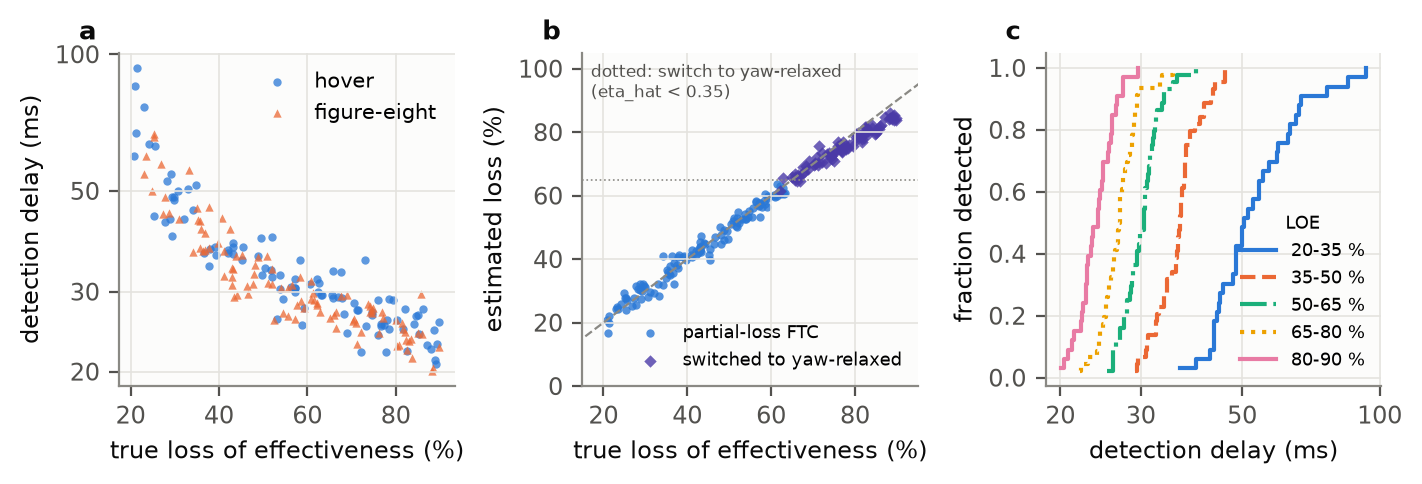
\includegraphics[width=\columnwidth]{fig_e2_fdi.png}
\caption{E2: detection delay versus LOE, estimated versus true LOE, and delay distribution per
magnitude bin (200 runs).}
\label{fig:e2}
\end{figure}

\textbf{Complete loss (E4, E5).} The passive controller lost all \resEFourN{} hover runs (median
\resEFourPassiveTtlS\,s after the failure) and all \resEFiveN{} figure-eight runs. The estimated
pipeline lost \resEFourEstLost/\resEFourN{} and \resEFiveEstLost/\resEFiveN, switching to yaw-relaxed
control a median \resEFourEstSwitchMs\,ms after the failure; the median peak deviation in hover was
\resEFourEstMaxdevCm\,cm (oracle \resEFourOracleMaxdevCm\,cm), the settled error
\resEFourEstSettledCm\,cm and the spin \resEFourEstSpin\,rad/s (Fig.~\ref{fig:e4},
Table~\ref{tab:e4}).

\begin{table*}[t]
\centering
\caption{E4/E5: complete loss of one rotor. Complete loss of one rotor (all four rotors in turn, several seeds each). Spin = mean $|\omega|$ over the last 2 s; switch delay = onset to yaw-relaxed control.}
\label{tab:e4}
\footnotesize
\setlength{\tabcolsep}{3pt}
\begin{adjustbox}{max width=\linewidth}
\begin{tabular}{lccccccc}
\toprule
case & baseline & lost & time to loss (s) & max dev. (cm) & settled (cm) & spin (rad/s) & switch delay (ms) \\
\midrule
hover & Passive & 32/32 & 0.30 & -- & -- & -- & -- \\
hover & Oracle & 0/32 & -- & 21.5 & 6.4 & 23.2 & 0 \\
hover & Estimated (proposed) & 0/32 & -- & 37.9 & 7.6 & 23.2 & 62 \\
figure-eight & Passive & 24/24 & 0.29 & -- & -- & -- & -- \\
figure-eight & Oracle & 0/24 & -- & 25.4 & 16.7 & 23.6 & 0 \\
figure-eight & Estimated (proposed) & 0/24 & -- & 39.2 & 18.3 & 23.6 & 62 \\
\bottomrule
\end{tabular}
\end{adjustbox}
\end{table*}


\begin{figure}[t]
\centering
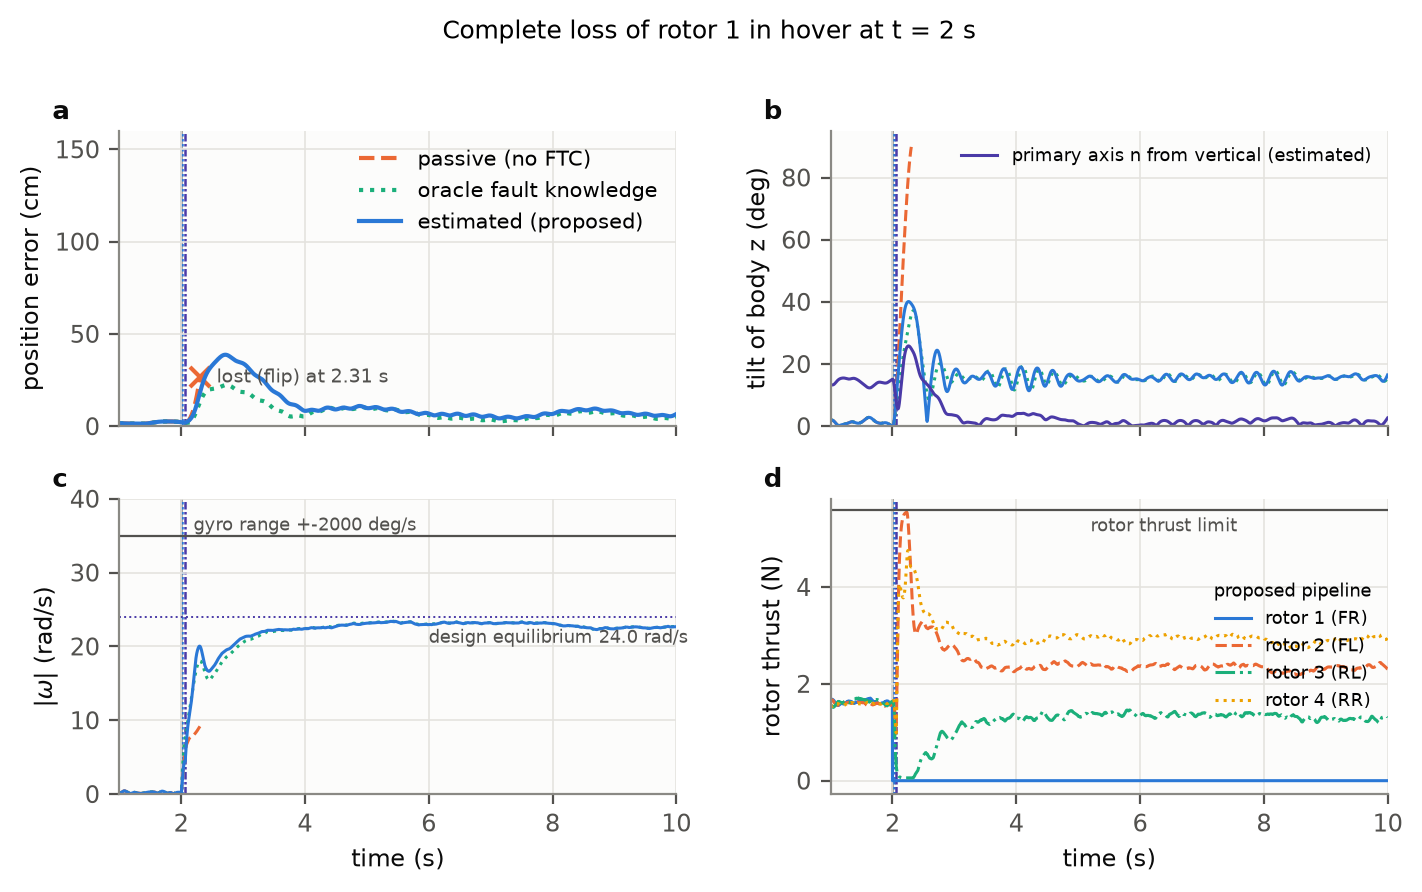
\includegraphics[width=\columnwidth]{fig_e4_complete_loss.png}
\caption{E4: complete loss of rotor 1 in hover: position error, tilt, spin rate and rotor thrusts.}
\label{fig:e4}
\end{figure}

\textbf{Limits (E6).} Generated from results/e6_robustness.json. Every run recovered over the whole tested range of rotational damping (0.25-2 x nominal) and inertia (0.7-1.4 x nominal). Runs were lost for: actuator delay (24 ms: 5/8 lost; tested 0-24 ms, nominal 2); motor time constant (80 ms: 8/8 lost, 100 ms: 8/8 lost; tested 15-100 ms, nominal 25); turbulence (3 x default: 5/8 lost, 4 x default: 6/8 lost; tested 0-4 x default, nominal 1).
 The design tolerates the inertia and damping
errors tested and motors up to 2.4$\times$ slower than assumed, but fails at 24\,ms actuator delay,
80\,ms motor time constant and 3$\times$ the default turbulence. All three act during the spin-up
transient, where the relaxed equilibrium leaves little margin and the body tilts by about
40$^\circ$ (Fig.~\ref{fig:e6}, Table~\ref{tab:e6}).

\begin{table}[t]
\centering
\caption{E6: robustness of complete-loss recovery. Complete loss in hover, estimated pipeline; the controller always assumes the nominal model.}
\label{tab:e6}
\footnotesize
\setlength{\tabcolsep}{3pt}
\begin{adjustbox}{max width=\linewidth}
\begin{tabular}{lc}
\toprule
true-system change & runs lost per value \\
\midrule
actuator delay (ms) & 0: 0/8, 2: 0/8, 4: 0/8, 8: 0/8, 12: 0/8, 16: 0/8, 20: 0/8, 24: 5/8 \\
motor time constant (ms) & 15: 0/8, 25: 0/8, 40: 0/8, 60: 0/8, 80: 8/8, 100: 8/8 \\
rotational damping (x) & 0.25: 0/8, 0.5: 0/8, 1: 0/8, 1.5: 0/8, 2: 0/8 \\
inertia (x) & 0.7: 0/8, 0.85: 0/8, 1: 0/8, 1.2: 0/8, 1.4: 0/8 \\
turbulence (x) & 0: 0/8, 1: 0/8, 2: 0/8, 3: 5/8, 4: 6/8 \\
\bottomrule
\end{tabular}
\end{adjustbox}
\end{table}


\begin{figure*}[t]
\centering
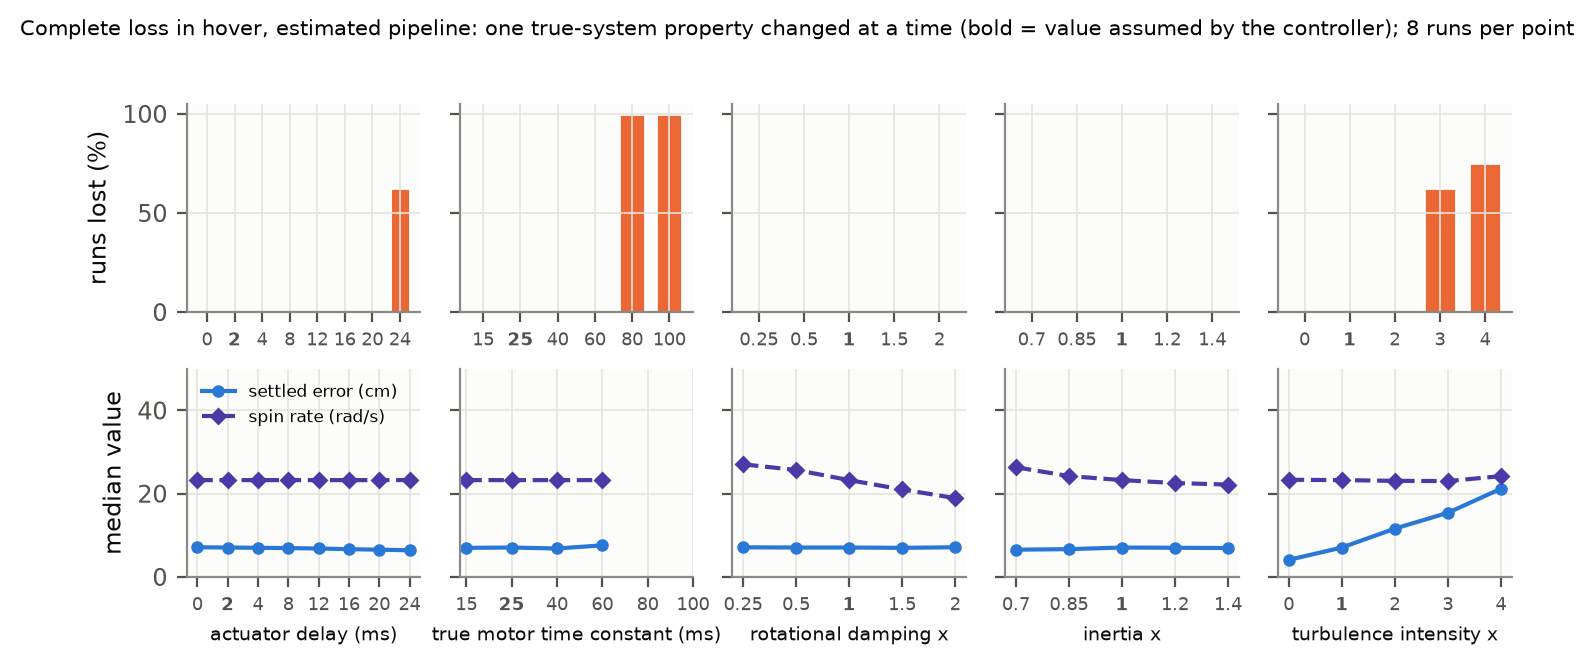
\includegraphics[width=0.85\textwidth]{fig_e6_robustness.png}
\caption{E6: robustness of complete-loss recovery (estimated pipeline) when one property of the
true system departs from the model.}
\label{fig:e6}
\end{figure*}

\begin{figure}[t]
\centering
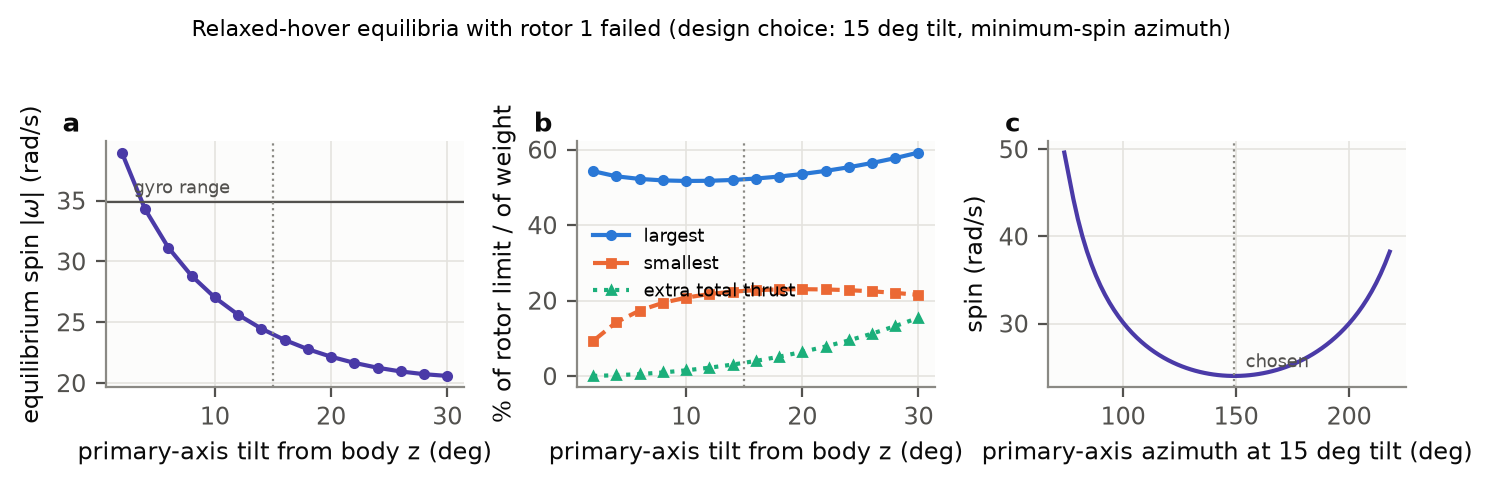
\includegraphics[width=\columnwidth]{fig_relaxed_family.png}
\caption{Relaxed-hover equilibria after the loss of rotor 1 versus primary-axis tilt and azimuth.}
\label{fig:family}
\end{figure}


\section{Discussion and limitations}
The results support the pipeline \emph{in simulation}: diagnosis is fast enough that the
partial-loss transient stays at the turbulence floor, and it is fast enough to hand a complete
loss to the yaw-relaxed controller within about 60\,ms. They do not show that it works on a
real 5-inch quadrotor. All parameters are assumed; the rotational damping that sets the spin
rate is the least certain, and the aerodynamics of a body spinning at more than 20\,rad/s is not
modelled. Real vibration is narrow-band and larger than the white noise used here, and the
turbulence model is a simple Gauss--Markov process, so the near-perfect detection numbers are
an upper bound. Faults are single steps; intermittent or growing damage, multiple faults and
sensor faults are not studied, the baseline assumes a fault-free initial hover, and the diagnoser
is not valid during the relaxed spin. Motion capture is assumed; GNSS and magnetometer
estimation while spinning is harder. Thresholds are calibrated from maxima of a few dozen
flights, which is a noisy statistic. The oracle is an upper bound on information, not on the
switching policy.

\section{Conclusion and next steps}
A model-based diagnoser (filtered rigid-body regression, Kalman filter, CUSUM bank) combined
with re-allocation for partial losses and a gain-scheduled yaw-relaxed controller for complete
losses recovered every simulated rotor fault in the main experiments, including complete losses during
3.3\,m/s flight; in the robustness sweeps it failed at large actuator delay, very slow motors and
strong turbulence. The next steps are PX4
SITL, offline evaluation on Betaflight blackbox logs of a real 5-inch quadrotor (including
identification of its parameters and the use of RPM telemetry), protected flight tests with a
weakened and then a cut propeller, and a comparison with INDI-based
FTC~\cite{smeur2016adaptive,sun2021incremental}.

\bibliographystyle{IEEEtran}
\bibliography{references}

\end{document}
